% Options for packages loaded elsewhere
\PassOptionsToPackage{unicode}{hyperref}
\PassOptionsToPackage{hyphens}{url}
\PassOptionsToPackage{dvipsnames,svgnames,x11names}{xcolor}
%
\documentclass[
  11pt,
]{article}
\usepackage{amsmath,amssymb}
\usepackage{iftex}
\ifPDFTeX
  \usepackage[T1]{fontenc}
  \usepackage[utf8]{inputenc}
  \usepackage{textcomp} % provide euro and other symbols
\else % if luatex or xetex
  \usepackage{unicode-math} % this also loads fontspec
  \defaultfontfeatures{Scale=MatchLowercase}
  \defaultfontfeatures[\rmfamily]{Ligatures=TeX,Scale=1}
\fi
\usepackage{lmodern}
\ifPDFTeX\else
  % xetex/luatex font selection
  \setmainfont[]{Latin Modern Roman}
  \setsansfont[]{Latin Modern Sans}
  \setmonofont[]{DejaVu Sans Mono}
\fi
% Use upquote if available, for straight quotes in verbatim environments
\IfFileExists{upquote.sty}{\usepackage{upquote}}{}
\IfFileExists{microtype.sty}{% use microtype if available
  \usepackage[]{microtype}
  \UseMicrotypeSet[protrusion]{basicmath} % disable protrusion for tt fonts
}{}
\makeatletter
\@ifundefined{KOMAClassName}{% if non-KOMA class
  \IfFileExists{parskip.sty}{%
    \usepackage{parskip}
  }{% else
    \setlength{\parindent}{0pt}
    \setlength{\parskip}{6pt plus 2pt minus 1pt}}
}{% if KOMA class
  \KOMAoptions{parskip=half}}
\makeatother
\usepackage{xcolor}
\usepackage[margin=25mm]{geometry}
\usepackage{longtable,booktabs,array}
\usepackage{calc} % for calculating minipage widths
% Correct order of tables after \paragraph or \subparagraph
\usepackage{etoolbox}
\makeatletter
\patchcmd\longtable{\par}{\if@noskipsec\mbox{}\fi\par}{}{}
\makeatother
% Allow footnotes in longtable head/foot
\IfFileExists{footnotehyper.sty}{\usepackage{footnotehyper}}{\usepackage{footnote}}
\makesavenoteenv{longtable}
\usepackage{graphicx}
\makeatletter
\def\maxwidth{\ifdim\Gin@nat@width>\linewidth\linewidth\else\Gin@nat@width\fi}
\def\maxheight{\ifdim\Gin@nat@height>\textheight\textheight\else\Gin@nat@height\fi}
\makeatother
% Scale images if necessary, so that they will not overflow the page
% margins by default, and it is still possible to overwrite the defaults
% using explicit options in \includegraphics[width, height, ...]{}
\setkeys{Gin}{width=\maxwidth,height=\maxheight,keepaspectratio}
% Set default figure placement to htbp
\makeatletter
\def\fps@figure{htbp}
\makeatother
\setlength{\emergencystretch}{3em} % prevent overfull lines
\providecommand{\tightlist}{%
  \setlength{\itemsep}{0pt}\setlength{\parskip}{0pt}}
\setcounter{secnumdepth}{5}
% definitions for citeproc citations
\NewDocumentCommand\citeproctext{}{}
\NewDocumentCommand\citeproc{mm}{%
  \begingroup\def\citeproctext{#2}\cite{#1}\endgroup}
\makeatletter
 % allow citations to break across lines
 \let\@cite@ofmt\@firstofone
 % avoid brackets around text for \cite:
 \def\@biblabel#1{}
 \def\@cite#1#2{{#1\if@tempswa , #2\fi}}
\makeatother
\newlength{\cslhangindent}
\setlength{\cslhangindent}{1.5em}
\newlength{\csllabelwidth}
\setlength{\csllabelwidth}{3em}
\newenvironment{CSLReferences}[2] % #1 hanging-indent, #2 entry-spacing
 {\begin{list}{}{%
  \setlength{\itemindent}{0pt}
  \setlength{\leftmargin}{0pt}
  \setlength{\parsep}{0pt}
  % turn on hanging indent if param 1 is 1
  \ifodd #1
   \setlength{\leftmargin}{\cslhangindent}
   \setlength{\itemindent}{-1\cslhangindent}
  \fi
  % set entry spacing
  \setlength{\itemsep}{#2\baselineskip}}}
 {\end{list}}
\usepackage{calc}
\newcommand{\CSLBlock}[1]{\hfill\break\parbox[t]{\linewidth}{\strut\ignorespaces#1\strut}}
\newcommand{\CSLLeftMargin}[1]{\parbox[t]{\csllabelwidth}{\strut#1\strut}}
\newcommand{\CSLRightInline}[1]{\parbox[t]{\linewidth - \csllabelwidth}{\strut#1\strut}}
\newcommand{\CSLIndent}[1]{\hspace{\cslhangindent}#1}
\usepackage{fancyhdr}
\usepackage{microtype}
\usepackage{needspace}
\usepackage{float}
\usepackage{caption}
\usepackage{seqsplit}
\captionsetup{font=small,labelfont=bf}
\floatplacement{figure}{H}
\pagestyle{fancy}
\fancyhf{}
\fancyhead[L]{\footnotesize\textsc{TACITUS · Context capsules}}
\fancyhead[R]{\footnotesize Research proposal TAC-2026-01 · v1.1}
\fancyfoot[C]{\small\thepage}
\setlength{\headheight}{14pt}
\setlength{\emergencystretch}{3em}
\setlength{\parskip}{5pt}
\setlength{\parindent}{0pt}
\AtBeginEnvironment{CSLReferences}{\small\interlinepenalty=10000}
\renewcommand{\headrulewidth}{0.3pt}
\AtBeginDocument{\hypersetup{pdftitle={TACITUS: Context Capsules, Artefacts, and Small Knowledge Graphs for AI Generation},pdfauthor={TACITUS},pdfsubject={Research proposal TAC-2026-01, version 1.1; not independently peer-reviewed},pdfkeywords={context capsules, artefacts, knowledge graphs, provenance, generation, evaluation}}}
\let\originalsection\section
\renewcommand{\section}{\Needspace{5\baselineskip}\originalsection}
\ifLuaTeX
  \usepackage{selnolig}  % disable illegal ligatures
\fi
\usepackage{bookmark}
\IfFileExists{xurl.sty}{\usepackage{xurl}}{} % add URL line breaks if available
\urlstyle{same}
\hypersetup{
  pdftitle={TACITUS: Context Capsules, Artefacts, and Small Knowledge Graphs for AI Generation},
  pdfauthor={TACITUS},
  colorlinks=true,
  linkcolor={teal},
  filecolor={Maroon},
  citecolor={Blue},
  urlcolor={teal},
  pdfcreator={LaTeX via pandoc}}

\title{TACITUS: Context Capsules, Artefacts, and Small Knowledge Graphs
for AI Generation}
\author{TACITUS}
\date{24 November 2026}

\begin{document}
\maketitle
\begin{abstract}
An analytical answer depends on the evidence selected for a task and on
working context that ordinary retrieval may leave behind: conditions,
source editions, unresolved objections, and reasons for earlier
decisions. We propose a portable context contract for TACITUS App, a
conversation and writing workspace. Context capsules bind selected
evidence and scoped working instructions; artefacts provide reusable
formats and retain the context of a work product. A small graph connects
passages, interpretations, qualifications, and review records, while an
explicit compiler prepares a bounded generation packet. The proposed
contribution is continuity across source updates and handovers, rather
than a claim that graph serialization intrinsically improves language
models. We specify the executable reference algorithm, its
dependency-preservation rules, and its limits. A reproducible comparison
of two NIST guidance editions demonstrates an identifier collision that
a context package must preserve. Six historical provider probes provide
mixed compatibility observations, including a graph-associated
overstatement. We then define comparisons with strong retrieval,
full-document context and an equivalent-information flat packet,
alongside a human-handover study. Outcomes include consequential
unsupported claims, retained qualifications, update accuracy, review
effort and total cost. The proposal establishes a testable design and
reproducible assembly examples; general generation-quality and
productivity benefits require the planned studies.
\end{abstract}

\textbf{Research proposal TAC-2026-01 · Version 1.1.} Published by
TACITUS. Independent peer review has not been completed. The efficacy
studies described here are proposed, not preregistered or run.

\textbf{Keywords:} context capsules; knowledge graphs;
retrieval-augmented generation; provenance; collaborative writing;
human--agent handover.

\section{Problem and candidate
contribution}\label{problem-and-candidate-contribution}

An analyst revising a policy note needs more than a relevant paragraph.
They may need the exact source edition, the condition limiting its
applicability, the reason a team retained cautious wording, and an
objection that remained unresolved. When this work moves to another
conversation, teammate or agent, these dependencies can disappear. The
recipient may produce a plausible answer while changing the meaning of
the earlier analysis.

TACITUS App organizes work around conversation and writing with
explicitly attached context. A \textbf{capsule} packages a purpose,
selected sources and working guidance. An \textbf{artefact} is a
reusable format, example or resulting work product. A \textbf{small
graph} records selected relationships among passages, interpretations,
conditions, discussions and review decisions. The graph supplies
structure to context selection and inspection; generation receives a
bounded packet, not an image of the graph or the entire knowledge store.

The candidate contribution is a portable contract connecting three
otherwise separable operations: selecting evidence for a request,
preserving the scope and review history of its interpretation, and
retaining that context when a work product is reused. This can be
implemented using ordinary records and typed edges. Its research value
depends on whether the contract improves continuity and accepted work,
rather than on a new graph class or foundation model.

The central question is: \textbf{Does reusable, reviewed context
preserve critical qualifications and team decisions across generation,
source updates and handover, at an acceptable total cost?} Three
hypotheses follow. Dependency-aware selection may prevent known
conditions from being separated from a claim. Explicit versions may help
recipients distinguish a source update from a changed recommendation.
Reusable context may reduce repeated explanation. Each has a competing
explanation: a careful ordinary note may achieve the same outcome, and
annotation and review may cost more than reuse saves.

\section{Relation to existing
research}\label{relation-to-existing-research}

Retrieval-augmented generation combines generation with retrievable
external information (\citeproc{ref-lewis2020}{Lewis et al. 2020}).
Long-context research shows that the position of relevant evidence can
affect its use (\citeproc{ref-liu2024}{Liu et al. 2024}). These motivate
testing selection and placement, but neither establishes that shorter
context or a particular graph improves every model. BM25 is an important
reproducible comparator (\citeproc{ref-robertson2009}{Robertson and
Zaragoza 2009}). BEIR further demonstrates why retrieval evaluation
should include varied architectures and the computational costs of
reranking (\citeproc{ref-thakur2021}{Thakur et al. 2021}); a
lexical-only baseline is insufficient to establish a practical advantage
over a capable contemporary system.

GraphRAG studies entity graphs and community summaries for corpus-level
questions (\citeproc{ref-edge2024}{Edge et al. 2024}). HippoRAG uses
knowledge graphs and Personalized PageRank for knowledge integration and
multi-hop retrieval (\citeproc{ref-gutierrez2024}{Jiménez Gutiérrez et
al. 2024}). LightRAG combines graph and vector representations with
retrieval at different levels (\citeproc{ref-guo2025}{Guo et al. 2025}).
TACITUS's public reference instead operates on authored mappings with
deterministic selection and explicit qualifications. The proposed
distinction is a reusable, review-scoped context contract across tasks
and actors. The evaluation must establish whether this integration adds
useful capability beyond these existing approaches.

Self-RAG studies learned conditional retrieval and reflection
(\citeproc{ref-asai2024}{Asai et al. 2024}), while ReAct studies
interleaving reasoning and task actions (\citeproc{ref-yao2023}{Yao et
al. 2023}). They motivate conditional evidence access and bounded agent
tools. The current TACITUS reference does not implement their learned
policies. LongMemEval's separation of cross-session reasoning, temporal
updates and abstention is directly relevant to handover
(\citeproc{ref-wu2025}{Wu et al. 2025}). Unlike automatic memory over an
entire interaction history, a capsule is deliberately selected and can
be reviewed for a stated purpose.

ALCE, Attributable to Identified Sources and FActScore motivate separate
measurements of citation quality, attributable statements and individual
factual claims (\citeproc{ref-gao2023}{Gao et al. 2023};
\citeproc{ref-rashkin2023}{Rashkin et al. 2023};
\citeproc{ref-min2023}{Min et al. 2023}). A resolving citation
identifier does not establish a supported paraphrase. PROV-O and SHACL
inform provenance and declared graph constraints
(\citeproc{ref-prov2013}{Lebo, Sahoo, and McGuinness 2013};
\citeproc{ref-shacl2017}{Knublauch and Kontokostas 2017}). Structural
validation and semantic correctness remain different questions.

Human--AI interaction research motivates correction and control over
adaptation (\citeproc{ref-amershi2019}{Amershi et al. 2019}); model
cards motivate explicit reporting of intended use and evaluation scope
(\citeproc{ref-mitchell2019}{Mitchell et al. 2019}). Model explanations
can also misrepresent the process producing an answer
(\citeproc{ref-turpin2023}{Turpin et al. 2023}). Accordingly,
\textbf{recorded reasoning} here means attributed discussion, analytical
warrants, objections and explanations of wording. It does not denote an
authenticated record of a model's private chain of thought.

\section{The portable context
contract}\label{the-portable-context-contract}

\subsection{Records, roles and review}\label{records-roles-and-review}

The contract distinguishes an external source statement, an
interpretation of it, a working instruction, and a generated result. A
source record identifies its edition and exact passages. An
interpretation preserves its author, modality, scope and supporting
spans. An instruction states how the team wants to perform the work. A
draft records its dependency on selected context and subsequent edits.
An example artefact can guide form without transferring its factual
contents to a new situation.

\Needspace{20\baselineskip}

\begin{longtable}[]{@{}
  >{\raggedright\arraybackslash}p{(\columnwidth - 4\tabcolsep) * \real{0.3333}}
  >{\raggedright\arraybackslash}p{(\columnwidth - 4\tabcolsep) * \real{0.3333}}
  >{\raggedright\arraybackslash}p{(\columnwidth - 4\tabcolsep) * \real{0.3333}}@{}}
\caption{Different record types carry different authority. Review is a
scoped judgment, not a universal truth label.}\tabularnewline
\toprule\noalign{}
\begin{minipage}[b]{\linewidth}\raggedright
Record
\end{minipage} & \begin{minipage}[b]{\linewidth}\raggedright
Required role in the contract
\end{minipage} & \begin{minipage}[b]{\linewidth}\raggedright
Failure it helps expose
\end{minipage} \\
\midrule\noalign{}
\endfirsthead
\toprule\noalign{}
\begin{minipage}[b]{\linewidth}\raggedright
Record
\end{minipage} & \begin{minipage}[b]{\linewidth}\raggedright
Required role in the contract
\end{minipage} & \begin{minipage}[b]{\linewidth}\raggedright
Failure it helps expose
\end{minipage} \\
\midrule\noalign{}
\endhead
\bottomrule\noalign{}
\endlastfoot
Source edition and passage & Stable identity, exact text, locator and
content pin & A quotation drawn from the wrong edition \\
Interpretation and qualification & Attributed claim, conditions,
exceptions and declared support & A permission presented as an
accomplished decision \\
Discussion and working decision & Contributor, stated rationale,
disagreement and intended use & A later writer losing why cautious
language was chosen \\
Capsule and artefact & Purpose, selected versions, output requirements
and reuse scope & A template's example content treated as new
evidence \\
Review and execution record & Exact reviewed content, authority,
dispatch selection and outcome & An old approval or an undispatched
preview mistaken for current acceptance \\
\end{longtable}

Human acceptance should bind to the exact interpretation, its source
dependencies and its intended use. The record should identify who
reviewed it, what they checked and what would require another review.
Source changes, revocation or a changed task can make an earlier
acceptance unsuitable for new use. The public reference emits proposed
interpretations; the App uses separate interpretation-review and
graph-activation contracts. A model critic supplies another
interpretation and cannot grant human acceptance.

\subsection{What the graph
contributes}\label{what-the-graph-contributes}

The graph records typed relationships such as a passage supporting an
interpretation, a condition qualifying it, or a discussion explaining a
wording decision. An ontology declares the vocabulary and permitted
relationships; a task layer selects the records and checks relevant to a
particular job. Neither supplies evidence absent from the source
collection.

``Small graph'' denotes a bounded task projection rather than a fixed
ideal number of nodes. The complete case graph and the model input are
different objects. More nodes may expose useful dependencies, but can
also add irrelevant material or amplify an annotation error. The
intended benefits are inspectable dependencies, explicit reuse and
targeted updates; improved output quality must be measured.

\begin{figure}
\centering
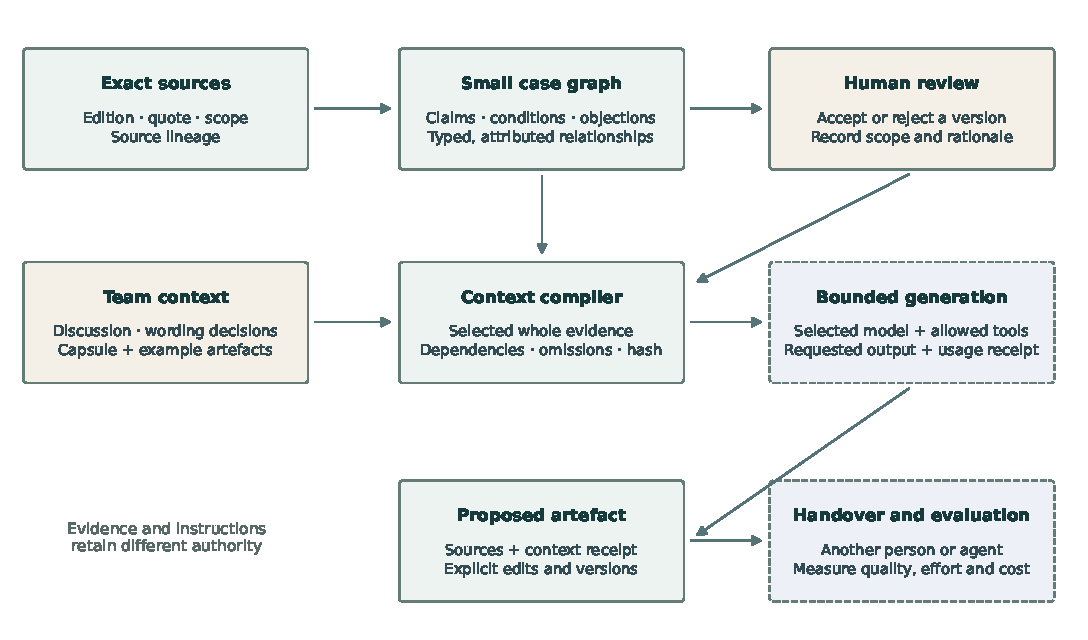
\includegraphics{figures/context-flow.pdf}
\caption{Context crosses the workflow through explicit records. The
compiler supplies a selected packet to generation. A recipient can
inspect evidence, working guidance and earlier decisions separately.
Dashed boxes indicate integrations or efficacy claims that require
further acceptance or evaluation.}
\end{figure}

The contract can be serialized as ordinary JSON, tables or prose. A
graph visualizer is a review interface. A graph index is a retrieval
mechanism. A graph serialization is a prompt representation. These are
distinct interventions, so the evaluation should vary them separately
rather than attributing every improvement in a complete pipeline to
``the graph.''

\section{Executable selection and
assembly}\label{executable-selection-and-assembly}

\subsection{Reference algorithm}\label{reference-algorithm}

The public reference is a credential-free Python implementation
operating on explicit source text and authored annotations. Its
implemented procedure is:

\begin{enumerate}
\def\labelenumi{\arabic{enumi}.}
\tightlist
\item
  \textbf{Validate the collection.} Require unique identities,
  attributed source URLs and content hashes. Check exact Unicode
  code-point quotation spans, relation domain/range and declared
  qualification spans. Every reference interpretation remains proposed.
\item
  \textbf{Select an authored task layer.} The layer declares eligible
  statements, required statements and reviewer checks. Optional BM25
  selection ranks quotation and interpretation text. Graph selection
  seeds from matches and expands through shared subject/object entities
  for at most two hops, recording inclusion reasons.
\item
  \textbf{Assemble required statements first.} A selected statement
  travels with its complete quotation, qualification records, source
  edition, relation and endpoint entities. The source register retains
  attribution and rights notes.
\item
  \textbf{Apply a byte gate.} Canonical UTF-8 JSON for the required
  packet must fit the budget. Otherwise assembly refuses. The core
  packer then considers optional statements in stable identifier order
  and includes a whole statement only when the resulting packet fits.
\item
  \textbf{Emit distinct outputs.} Return the full selected-layer graph,
  bounded capsule, evidence worksheet, omissions and a checksum receipt.
  The App import bundle additionally carries the exact source collection
  and ontology for independent validation.
\end{enumerate}

This describes actual code rather than an unspecified optimal utility
function. The graph option changes eligible selection; the core packer
is not a learned ranker and does not solve a globally optimal packing
problem. Required layer statements remain mandatory, even if their count
exceeds a requested optional-selection limit; the complete-packet byte
gate still applies. The implementation must be evaluated at these actual
boundaries.

Three useful invariants are enforced: a retained quotation matches its
pinned source span; a declared required qualification is retained with
its statement; and a mandatory packet that exceeds budget is refused as
a whole. These invariants cover declared dependencies. They cannot
identify an exception that was never annotated, determine legal
applicability or establish the truth of an interpretation. Such errors
require separate source review and tests.

\subsection{App projection and
dispatch}\label{app-projection-and-dispatch}

The reviewed App source has a separate selector using lexical
inverse-frequency matching, selected graph anchors and adjacent
qualification handling. Its graph-context contract bounds selection to
four graphs, 128 nodes, 256 edges, 24 KiB of graph context and 65,536
bytes for the complete packet. These are operational limits, not
experimentally selected optima. Python code-point offsets are mapped to
the App's UTF-16 convention against exact original text.

The proposed dispatch contract retains the selected object and source
versions, graph selection, packet hash, requested and reported model
identity, settings, observed usage and resulting artefact. Conversation
and Writing should share the same evidence contract. A local model may
be another generator behind it, but local inference and hosted storage
have separate data and resource boundaries. Historical receipts remain
identifiable after a source update; new dispatch checks current access
and eligible review state.

\section{Source-update and handover
case}\label{source-update-and-handover-case}

\subsection{A real identifier
collision}\label{a-real-identifier-collision}

The archived April 2024 draft and July 2024 final editions of NIST AI
600-1 provide a concrete source-maintenance problem
(\citeproc{ref-nistdraft2024}{National Institute of Standards and
Technology 2024a}, \citeproc{ref-nistfinal2024}{2024b}). In their
MEASURE 2.5 tables, the action advising source-and-citation verification
has the same wording, including pre-deployment measurement and ongoing
monitoring. Its identifier changes from \textbf{MS-2.5-008} in the draft
to \textbf{MS-2.5-003} in the final. The draft's \textbf{MS-2.5-003}
describes a different security-assessment practice.

\Needspace{20\baselineskip}

\begin{longtable}[]{@{}
  >{\raggedright\arraybackslash}p{(\columnwidth - 4\tabcolsep) * \real{0.3333}}
  >{\raggedright\arraybackslash}p{(\columnwidth - 4\tabcolsep) * \real{0.3333}}
  >{\raggedright\arraybackslash}p{(\columnwidth - 4\tabcolsep) * \real{0.3333}}@{}}
\caption{The identifier alone is insufficient. This is a comparison of
specified historical editions, not an assessment of all current NIST
guidance.}\tabularnewline
\toprule\noalign{}
\begin{minipage}[b]{\linewidth}\raggedright
Pinned edition
\end{minipage} & \begin{minipage}[b]{\linewidth}\raggedright
Identifier
\end{minipage} & \begin{minipage}[b]{\linewidth}\raggedright
Practice in the captured passage
\end{minipage} \\
\midrule\noalign{}
\endfirsthead
\toprule\noalign{}
\begin{minipage}[b]{\linewidth}\raggedright
Pinned edition
\end{minipage} & \begin{minipage}[b]{\linewidth}\raggedright
Identifier
\end{minipage} & \begin{minipage}[b]{\linewidth}\raggedright
Practice in the captured passage
\end{minipage} \\
\midrule\noalign{}
\endhead
\bottomrule\noalign{}
\endlastfoot
April draft, printed p.~39 & MS-2.5-008 & Source-and-citation
verification \\
July final, printed p.~31 & MS-2.5-003 & The same verification
wording \\
April draft, printed p.~39 & MS-2.5-003 & Security assessments and
integrity audits \\
\end{longtable}

An analyst updating an internal review note should change the
edition-bound citation while retaining the verification practice and its
timing. Looking up only the final identifier in the draft would retrieve
a different practice. A useful handover therefore carries all three
spans and the authored rationale: change the reference, retain the cited
advice, and distinguish the same-number collision. NIST describes
suggested guidance; the example must preserve that modality rather than
turn it into a statutory obligation.

\begin{figure}
\centering
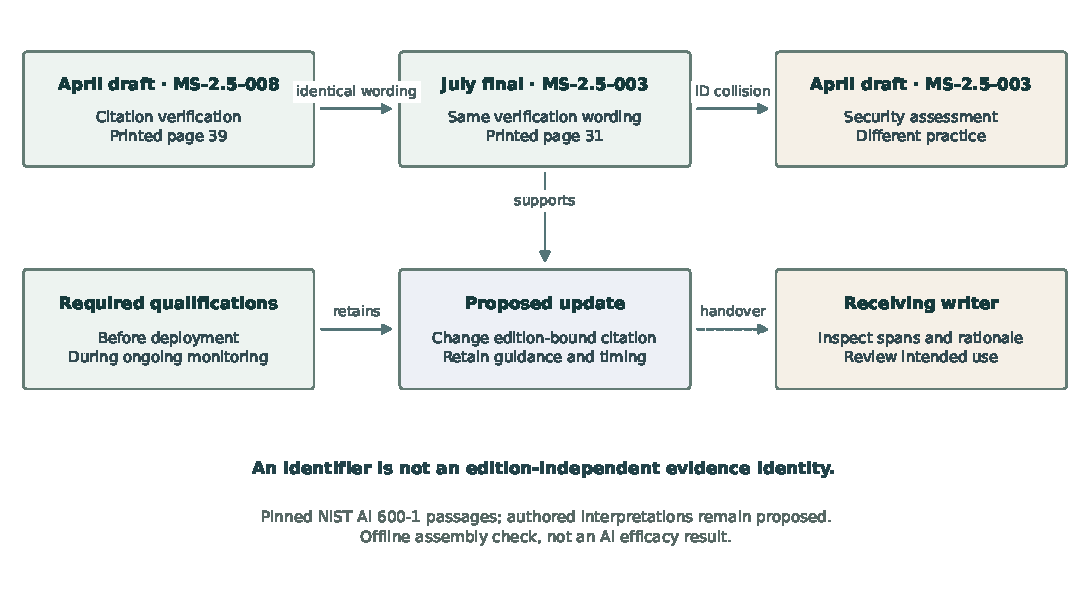
\includegraphics{figures/edition-handover.pdf}
\caption{Edition-bound identities prevent the same identifier from
silently linking to a different practice. The source comparison supports
an authored update recommendation; the receiving writer still reviews
the recommendation and its intended use.}
\end{figure}

The publication replay checks the exact captured text hashes, offsets
and wording equality, then rebuilds a capsule containing three proposed
statements from two source records. The recorded packet uses 4,726
canonical UTF-8 bytes at a 24,000-byte budget. Its source capture
records official PDF hashes and extraction rules; optional verification
against those PDFs is available in the reference fixture. The replay
establishes this assembly result, not better AI generation or saved
analyst time.

A careful ordinary note could express the same information. That is
precisely why the evaluation must compare a capsule with a well-prepared
note, not merely with a question lacking the relevant context. The case
is development material already inspected by the builders and must be
excluded from held-out efficacy testing. The package's
\texttt{source-edition-case.json} makes the source-to-interpretation
mapping inspectable.

\section{Available evidence and its
scope}\label{available-evidence-and-its-scope}

Source validation, reference assembly and import contracts can be
exercised without a model. The reviewed App source also includes context
previews, saved objects, graph selection and interpretation-review
records. The documented hosted release keeps generation paused; a
configured model or billing guard is not end-to-end execution
acceptance. This proposal does not establish a fresh audit of every
deployed App feature.

Six historical direct Cloudflare provider requests on 23 November 2026
used one synthetic renewal question, with flat and graph-annotated arms
for three model families. All six returned valid response structures and
resolving citation identifiers. Qualitative review found that Gemma's
flat answer omitted a required condition, while its graph-assisted
answer retained it; GPT-OSS retained the material distinctions in both
arms; GLM's graph-assisted answer strengthened the action's procedural
status and omitted duration.

These observations were post-hoc, unblinded and AI-assisted. The graph
arm added annotations, including a potentially misleading
proposed-action label, so the arms were not information-equivalent. The
recordings support provider compatibility and identify failure cases.
They neither estimate an average quality effect nor validate the
deployed App route. Their exact inputs, final answers, usage and hashes
remain in the historical public record; this revision makes no new model
calls.

\section{Proposed evaluation}\label{proposed-evaluation}

\subsection{Comparators that can challenge the
claim}\label{comparators-that-can-challenge-the-claim}

The primary practical comparison should use a strong retrieval system:
lexical and dense candidates with a registered fusion and reranking
procedure, selected on development collections and frozen before
testing. Its actual retriever, embedding model, reranker, index cost and
token limits must be disclosed. BM25 remains a useful inexpensive
ablation rather than the sole primary comparator.

\Needspace{20\baselineskip}

\begin{longtable}[]{@{}
  >{\raggedright\arraybackslash}p{(\columnwidth - 4\tabcolsep) * \real{0.3333}}
  >{\raggedright\arraybackslash}p{(\columnwidth - 4\tabcolsep) * \real{0.3333}}
  >{\raggedright\arraybackslash}p{(\columnwidth - 4\tabcolsep) * \real{0.3333}}@{}}
\caption{D--B measures the complete pipeline, including annotation
effort. D--C is a representation diagnostic. C must retain relation
meaning; it must not become a deliberately weaker answer context.
Compare A only on a prespecified common eligible subset.}\tabularnewline
\toprule\noalign{}
\begin{minipage}[b]{\linewidth}\raggedright
Arm
\end{minipage} & \begin{minipage}[b]{\linewidth}\raggedright
Information and preparation
\end{minipage} & \begin{minipage}[b]{\linewidth}\raggedright
Question addressed
\end{minipage} \\
\midrule\noalign{}
\endfirsthead
\toprule\noalign{}
\begin{minipage}[b]{\linewidth}\raggedright
Arm
\end{minipage} & \begin{minipage}[b]{\linewidth}\raggedright
Information and preparation
\end{minipage} & \begin{minipage}[b]{\linewidth}\raggedright
Question addressed
\end{minipage} \\
\midrule\noalign{}
\endhead
\bottomrule\noalign{}
\endlastfoot
A: full context and note & Eligible source documents plus a carefully
prepared working note & Can ordinary context already solve the task? \\
B: strong retrieval & Frozen hybrid retrieval, reranking and ordinary
source metadata & Does the complete capsule pipeline improve useful
work? \\
C: reviewed flat packet & The same selected evidence, instructions,
qualifications and relation meanings as D, rendered linearly & What does
reviewed content achieve without graph serialization? \\
D: capsule and graph & The reviewed packet with explicit typed
relationships and dependency records & Does the proposed integration and
representation add value? \\
\end{longtable}

Within paired contrasts, freeze the model snapshot, source pool, task,
system instructions, answer format, decoding settings and output cap.
Report actual input tokens and information content, and include
matched-budget sensitivity analyses when encodings differ. A hosted
model and a runnable local model can form separate blocks after their
routes and resources are accepted. Full-document cases must be
identified before results, and model substitutions require a new
recorded block.

\subsection{Tasks, review and analysis}\label{tasks-review-and-analysis}

Start with at least 24 feasibility tasks across disjoint collections. A
provisional confirmatory design is 120 tasks from 30 collections; its
final size requires clustered power analysis from feasibility estimates
before the held-out set is unlocked. Register the resulting sample,
stopping rule, primary contrast, exclusions and analysis. These are
planning quantities, not a completed or adequately powered trial.

An independent panel should create held-out questions and prelist their
critical facts, qualifications, source editions and acceptable
abstentions. Include analytical writing, conflicting accounts, source
updates, changed identifiers, multilingual modality and missing
evidence. Freeze case annotations before builders see held-out questions
or reference answers. Separate source preparation, retrieval and
generation so the analysis can locate the stage of a failure.

The primary endpoint is \textbf{clean task completion}: a valid
completion handles every critical point, including justified abstention
where required, and contains no consequential unsupported claim. Failed,
missing and timed-out attempts remain assigned tasks. Two independent
domain reviewers assess shuffled, de-identified answers using the frozen
rubric, with adjudication and recorded disagreements. Content can reveal
an arm despite removed labels; this limitation should be assessed.
Automated judges are secondary and require calibration against human
judgments.

\Needspace{7\baselineskip}

For paired task \(i\), let \(Y_{ia}\) denote clean completion under arm
\(a\). The primary effect is

\[
\widehat{\Delta}=\frac{1}{n}\sum_{i=1}^{n}(Y_{iD}-Y_{iB}).
\]

Use uncertainty intervals resampled at the source-collection level,
retaining complete clusters. Report effect sizes, all failed runs and
reviewer agreement. Treat D--C, eligible A comparisons and subgroup
analyses as secondary, with prespecified multiplicity handling or
exploratory labels. Secondary measures include supported-claim precision
and coverage together, retained conditions, actor/edition accuracy,
correct updates, critical-span retrieval and useful revisions. Precision
alone can reward an incomplete answer.

\subsection{Mechanisms, handover and
cost}\label{mechanisms-handover-and-cost}

Vary context budget, evidence position and graph size within actual
runtime limits. Remove prior discussion, typed organization or
dependency closure in separate ablations. Test incorrect annotations,
same-name actors and outdated review records. A graph can spread a
mistaken interpretation more consistently; adverse cases are a central
outcome, not noise to discard.

For handover, give a recipient an unfinished analysis after another
analyst establishes its context. Compare ordinary documents and history
with a capsule and artefact; balance recipient experience and task
assignment, using separate cases to reduce learning carryover. Measure
rationale-recovery time, consequential errors, clarifying questions,
recognition of unresolved objections and time to an accepted result. A
bounded agent can be a later recipient condition under the same allowed
evidence and actions.

Count preparation, annotation, review, indexing, retrieval, inference,
failures, maintenance and revision. Attribute one-time construction
costs across observed reuse rather than assuming unlimited future reuse.
Report quality at the same budget and total cost at the same acceptance
threshold. A system that saves input tokens but increases review time
may have no economic advantage. The handover study requires consent and
a fixed analysis protocol before participant work.

\section{Engineering boundaries and
deployment}\label{engineering-boundaries-and-deployment}

The initial design needs versioned records, exact-source storage and
bounded traversal; a specialized graph database is optional. More
infrastructure should follow measured workload needs. Schema checks
should identify the operation performed---such as quotation
identity---rather than present an undifferentiated trust score. Review
authority, source rights, access scope and retention remain application
responsibilities.

Retrieved material can contain indirect prompt injection
(\citeproc{ref-greshake2023}{Greshake et al. 2023}). Source text and
graph annotations must remain task data, with server-side tool
permissions and access controls. Separate integrity tests should cover
tampered spans, forged approval metadata, revoked access, oversized
packets and uncertain duplicate dispatch. Multiple model stages do not
create independent evidence, and generated explanations remain
attributed proposals.

Deployment should progress through packet integrity, authenticated
attachment and revocation, bounded dispatch and accounting, held-out
evaluation, and measured team pilots. Software tests establish specific
contracts, while truthfulness, legal applicability and customer value
require separate evidence. Recurring tasks may amortize preparation;
ordinary retrieval may better serve one-off questions.

\section{Conclusion and disclosures}\label{conclusion-and-disclosures}

TACITUS proposes a reusable context contract across evidence selection,
generation, updates and handover. Its reference algorithm enforces
declared identity and qualification rules; the NIST case demonstrates a
versioning problem. Graph organization, output quality and productivity
remain empirical questions for the proposed comparisons.

TACITUS is the author, developer and publisher, with a commercial
interest. Proposal TAC-2026-01, version 1.1 has not undergone
independent peer review; confirmatory studies have not been run or
preregistered. AI assisted writing, source/code inspection and
historical qualitative review, not independent domain review. Literature
selection was targeted, not systematic. No endorsement or registered DOI
is claimed.

\section*{Appendix. Materials and
reproduction}\label{appendix.-materials-and-reproduction}
\addcontentsline{toc}{section}{Appendix. Materials and reproduction}

The package includes the manuscript, twenty-one references, vector
figures, source-edition case, proposed protocol, implementation-status
record and checksums. The earlier synthetic compatibility replay remains
separate development material. Private App code and customer documents
are excluded. Source rights, NIST attribution and capture rights notes
are retained.

Reviewed public reference commit:
\texttt{\seqsplit{9fa96f66593902c5631efc391ef449a9c724b958}}. Private
App source-review pin:
\texttt{\seqsplit{2f11863ed506502a2bc508840a8e4d30ff69f15f}}; this does
not publicly reproduce the application. From the repository root, Python
3.11+ runs \texttt{research/context-capsules/v1.1/replay.py} and
\texttt{verify.py} without credentials or inference. Publication
rebuilding also requires Matplotlib, Pandoc/citeproc and XeLaTeX.
Version 1.0 remains archived.

\section*{References}\label{references}
\addcontentsline{toc}{section}{References}

\phantomsection\label{refs}
\begin{CSLReferences}{1}{0}
\bibitem[\citeproctext]{ref-amershi2019}
Amershi, Saleema, Dan Weld, Mihaela Vorvoreanu, Adam Fourney, Besmira
Nushi, Penny Collisson, Jina Suh, et al. 2019. {``Guidelines for
Human-AI Interaction.''} In \emph{Proceedings of the 2019 CHI Conference
on Human Factors in Computing Systems}.
\url{https://doi.org/10.1145/3290605.3300233}.

\bibitem[\citeproctext]{ref-asai2024}
Asai, Akari, Zeqiu Wu, Yizhong Wang, Avirup Sil, and Hannaneh
Hajishirzi. 2024. {``Self-RAG: Learning to Retrieve, Generate, and
Critique Through Self-Reflection.''} In \emph{International Conference
on Learning Representations}.
\url{https://proceedings.iclr.cc/paper_files/paper/2024/hash/25f7be9694d7b32d5cc670927b8091e1-Abstract-Conference.html}.

\bibitem[\citeproctext]{ref-edge2024}
Edge, Darren, Ha Trinh, Newman Cheng, Joshua Bradley, Alex Chao, Apurva
Mody, Steven Truitt, Dasha Metropolitansky, Robert Osazuwa Ness, and
Jonathan Larson. 2024. {``From Local to Global: A Graph RAG Approach to
Query-Focused Summarization.''} arXiv preprint 2404.16130.
\url{https://arxiv.org/abs/2404.16130}.

\bibitem[\citeproctext]{ref-gao2023}
Gao, Tianyu, Howard Yen, Jiatong Yu, and Danqi Chen. 2023. {``Enabling
Large Language Models to Generate Text with Citations.''} In
\emph{Proceedings of the 2023 Conference on Empirical Methods in Natural
Language Processing}, 6465--88.
\url{https://doi.org/10.18653/v1/2023.emnlp-main.398}.

\bibitem[\citeproctext]{ref-greshake2023}
Greshake, Kai, Sahar Abdelnabi, Shailesh Mishra, Christoph Endres,
Thorsten Holz, and Mario Fritz. 2023. {``Not What You've Signed Up For:
Compromising Real-World LLM-Integrated Applications with Indirect Prompt
Injection.''} arXiv preprint 2302.12173.
\url{https://arxiv.org/abs/2302.12173}.

\bibitem[\citeproctext]{ref-guo2025}
Guo, Zirui, Lianghao Xia, Yanhua Yu, Tu Ao, and Chao Huang. 2025.
{``LightRAG: Simple and Fast Retrieval-Augmented Generation.''} In
\emph{Findings of the Association for Computational Linguistics: EMNLP
2025}, 10746--61.
\url{https://doi.org/10.18653/v1/2025.findings-emnlp.568}.

\bibitem[\citeproctext]{ref-gutierrez2024}
Jiménez Gutiérrez, Bernal, Yiheng Shu, Yu Gu, Michihiro Yasunaga, and Yu
Su. 2024. {``HippoRAG: Neurobiologically Inspired Long-Term Memory for
Large Language Models.''} In \emph{Advances in Neural Information
Processing Systems}. Vol. 37.
\url{https://proceedings.neurips.cc/paper_files/paper/2024/hash/6ddc001d07ca4f319af96a3024f6dbd1-Abstract-Conference.html}.

\bibitem[\citeproctext]{ref-shacl2017}
Knublauch, Holger, and Dimitris Kontokostas. 2017. {``Shapes Constraint
Language (SHACL).''} W3C Recommendation. World Wide Web Consortium.
\url{https://www.w3.org/TR/2017/REC-shacl-20170720/}.

\bibitem[\citeproctext]{ref-prov2013}
Lebo, Timothy, Satya Sahoo, and Deborah McGuinness. 2013. {``PROV-O: The
PROV Ontology.''} W3C Recommendation. World Wide Web Consortium.
\url{https://www.w3.org/TR/prov-o/}.

\bibitem[\citeproctext]{ref-lewis2020}
Lewis, Patrick, Ethan Perez, Aleksandra Piktus, Fabio Petroni, Vladimir
Karpukhin, Naman Goyal, Heinrich Küttler, et al. 2020.
{``Retrieval-Augmented Generation for Knowledge-Intensive NLP Tasks.''}
In \emph{Advances in Neural Information Processing Systems}. Vol. 33.
\url{https://proceedings.neurips.cc/paper/2020/hash/6b493230205f780e1bc26945df7481e5-Abstract.html}.

\bibitem[\citeproctext]{ref-liu2024}
Liu, Nelson F., Kevin Lin, John Hewitt, Ashwin Paranjape, Michele
Bevilacqua, Fabio Petroni, and Percy Liang. 2024. {``Lost in the Middle:
How Language Models Use Long Contexts.''} \emph{Transactions of the
Association for Computational Linguistics} 12: 157--73.
\url{https://doi.org/10.1162/tacl_a_00638}.

\bibitem[\citeproctext]{ref-min2023}
Min, Sewon, Kalpesh Krishna, Xinxi Lyu, Mike Lewis, Wen-tau Yih, Pang
Koh, Mohit Iyyer, Luke Zettlemoyer, and Hannaneh Hajishirzi. 2023.
{``FActScore: Fine-Grained Atomic Evaluation of Factual Precision in
Long Form Text Generation.''} In \emph{Proceedings of the 2023
Conference on Empirical Methods in Natural Language Processing},
12076--100. \url{https://doi.org/10.18653/v1/2023.emnlp-main.741}.

\bibitem[\citeproctext]{ref-mitchell2019}
Mitchell, Margaret, Simone Wu, Andrew Zaldivar, Parker Barnes, Lucy
Vasserman, Ben Hutchinson, Elena Spitzer, Inioluwa Deborah Raji, and
Timnit Gebru. 2019. {``Model Cards for Model Reporting.''} In
\emph{Proceedings of the Conference on Fairness, Accountability, and
Transparency}, 220--29. \url{https://doi.org/10.1145/3287560.3287596}.

\bibitem[\citeproctext]{ref-nistdraft2024}
National Institute of Standards and Technology. 2024a. {``Artificial
Intelligence Risk Management Framework: Generative Artificial
Intelligence Profile (Initial Public Draft).''} NIST AI 600-1. National
Institute of Standards and Technology.
\url{https://airc.nist.gov/docs/NIST.AI.600-1.GenAI-Profile.ipd.pdf}.

\bibitem[\citeproctext]{ref-nistfinal2024}
---------. 2024b. {``Artificial Intelligence Risk Management Framework:
Generative Artificial Intelligence Profile.''} NIST AI 600-1. National
Institute of Standards and Technology.
\url{https://doi.org/10.6028/NIST.AI.600-1}.

\bibitem[\citeproctext]{ref-rashkin2023}
Rashkin, Hannah, Vitaly Nikolaev, Matthew Lamm, Lora Aroyo, Michael
Collins, Dipanjan Das, Slav Petrov, Gaurav Singh Tomar, Iulia Turc, and
David Reitter. 2023. {``Measuring Attribution in Natural Language
Generation Models.''} \emph{Computational Linguistics} 49 (4): 777--840.
\url{https://doi.org/10.1162/coli_a_00486}.

\bibitem[\citeproctext]{ref-robertson2009}
Robertson, Stephen, and Hugo Zaragoza. 2009. {``The Probabilistic
Relevance Framework: BM25 and Beyond.''} \emph{Foundations and Trends in
Information Retrieval}. \url{https://doi.org/10.1561/1500000019}.

\bibitem[\citeproctext]{ref-thakur2021}
Thakur, Nandan, Nils Reimers, Andreas Rücklé, Abhishek Srivastava, and
Iryna Gurevych. 2021. {``BEIR: A Heterogeneous Benchmark for Zero-Shot
Evaluation of Information Retrieval Models.''} In \emph{Proceedings of
the Neural Information Processing Systems Track on Datasets and
Benchmarks}. Vol. 1.
\url{https://datasets-benchmarks-proceedings.neurips.cc/paper_files/paper/2021/hash/65b9eea6e1cc6bb9f0cd2a47751a186f-Abstract-round2.html}.

\bibitem[\citeproctext]{ref-turpin2023}
Turpin, Miles, Julian Michael, Ethan Perez, and Samuel Bowman. 2023.
{``Language Models Don't Always Say What They Think: Unfaithful
Explanations in Chain-of-Thought Prompting.''} In \emph{Advances in
Neural Information Processing Systems}. Vol. 36.
\url{https://papers.nips.cc/paper/2023/hash/ed3fea9033a80fea1376299fa7863f4a-Abstract-Conference.html}.

\bibitem[\citeproctext]{ref-wu2025}
Wu, Di, Hongwei Wang, Wenhao Yu, Yuwei Zhang, Kai-Wei Chang, and Dong
Yu. 2025. {``LongMemEval: Benchmarking Chat Assistants on Long-Term
Interactive Memory.''} In \emph{International Conference on Learning
Representations}. \url{https://arxiv.org/abs/2410.10813}.

\bibitem[\citeproctext]{ref-yao2023}
Yao, Shunyu, Jeffrey Zhao, Dian Yu, Nan Du, Izhak Shafran, Karthik
Narasimhan, and Yuan Cao. 2023. {``ReAct: Synergizing Reasoning and
Acting in Language Models.''} In \emph{International Conference on
Learning Representations}. \url{https://arxiv.org/abs/2210.03629}.

\end{CSLReferences}

\end{document}
